\chapter{Potentiometer Linearity}\label{app:potentiometerLin} 
\textbf{Name: Group 630}\\
\textbf{Date: 15/03 - 2016}

\subsubsection{Purpose}
Finding the linearity accuracy of the potentiometer.

\subsubsection{Setup}
\begin{figure}[H]
	\centering
	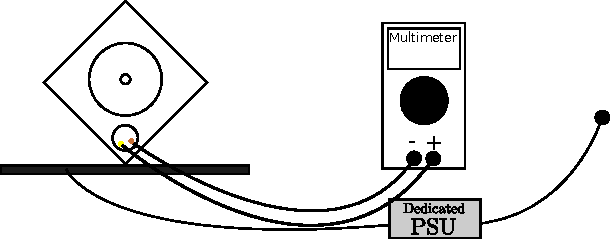
\includegraphics[scale=1]{figures/LabSetupLinearityTest.pdf}
	\caption{Setup diagram}
	\label{LabSetupRangeTest}
\end{figure}\vspace{-5mm}

\subsubsection{List of Equipment}
\begin{table}[H]
	\begin{tabular}{|l|l|p{4.3cm}|}
		\hline%------------------------------------------------------------------------------------------------------------
		\textbf{Instrument}                                  &  \textbf{AAU-no.}  &  \textbf{Type}                       \\
		\hline%------------------------------------------------------------------------------------------------------------
		Multimeter                                           &  60760           &  Fluke 189 Multimeter		                   \\
		\hline%------------------------------------------------------------------------------------------------------------
		Dedicated Power Supply of Cubli \small{(24 V - 3 A)} &  AAU3                   &  XP Power, AEB70US24                 \\
		\hline%------------------------------------------------------------------------------------------------------------
		Digital Protractor                                   &  None               & CMT Orange Tools     \\
		\hline%------------------------------------------------------------------------------------------------------------
	\end{tabular}
\end{table}

\subsubsection{Procedure}
\begin{enumerate}
	\item Make the setup with connections as seen on \figref{LabSetupRangeTest}, with minus on brown and plus on yellow of the potentiometer.
	\item Setting the multimeter to measure DC mV.
	\item Balance the frame in upright equilibrium position measuring the angle and voltage.
	\item Measuring  the voltage of the potentiometer around Equilibrium point and also min and max angle voltage for every 10 degree.
\end{enumerate}


\subsubsection{Results}
\begin{table}[H]
	\begin{tabular}{|l|l|p{4.3cm}|}
		\hline%------------------------------------------------------------------------------------------------------------
		\textbf{Angle from equilibrium in degrees}    &  \textbf{mV}         \\
		\hline%------------------------------------------------------------------------------------------------------------
		-41,7                                         & 0,066               \\
		\hline%------------------------------------------------------------------------------------------------------------
		-40,0 										  & 0,067               \\
		\hline%------------------------------------------------------------------------------------------------------------
		-38,5                              			  & 4,25               \\
		\hline%------------------------------------------------------------------------------------------------------------
		-30,0                              			  & 50,55               \\
		\hline%------------------------------------------------------------------------------------------------------------
		-20,0                                         & 103,66               \\
		\hline%------------------------------------------------------------------------------------------------------------
		-10,0 										  & 159,20               \\
		\hline%------------------------------------------------------------------------------------------------------------
		0                               			  & 213,64               \\
		\hline%------------------------------------------------------------------------------------------------------------
		10,0                                          & 264,66               \\
		\hline%------------------------------------------------------------------------------------------------------------
		20,0 										  & 317,95               \\
		\hline%------------------------------------------------------------------------------------------------------------
		30,0                              			  & 370,74               \\
		\hline%------------------------------------------------------------------------------------------------------------
		40,0                                          & 425,10               \\
		\hline%------------------------------------------------------------------------------------------------------------
		48,65 										  & 472,11               \\
		\hline%------------------------------------------------------------------------------------------------------------		
	\end{tabular}
\end{table}


\subsubsection{Results}
Result of the test shows that below -39,5 degrees the potentiometer has a dead area. The dead area might come from the continuous rotation of the potentiometer, since the measurement are very near to this point where the potentiometer changes. The area have at dead span from 5 to 10 degrees.

The graph shows the measured values according to angle.

\begin{figure}[H] 
	\centering 
	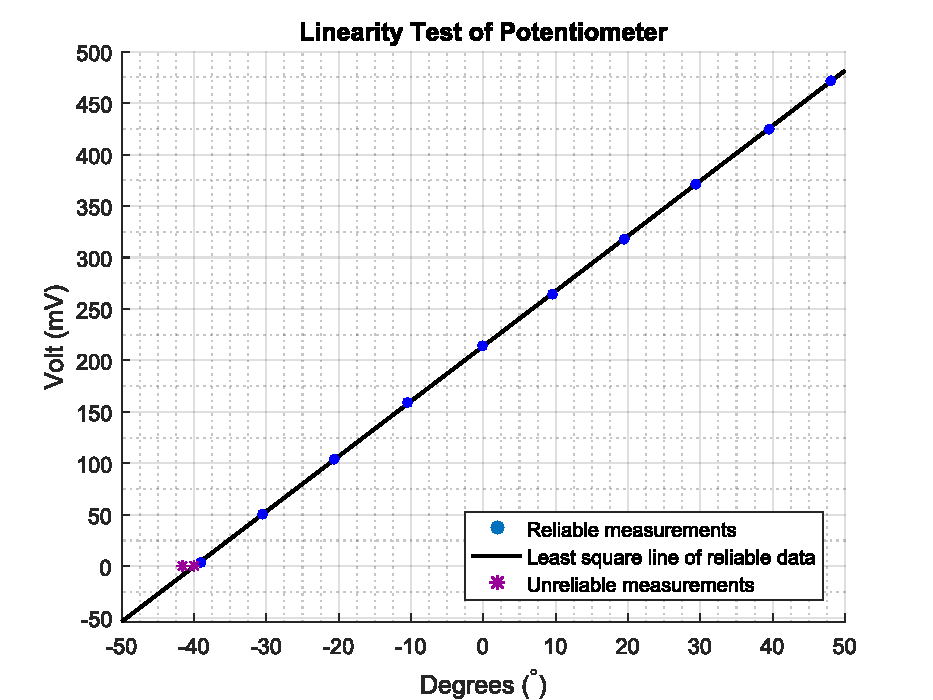
\includegraphics[scale=0.7]{figures/linearityOfPotmeterTest2-1}
	\caption{Raw test data plot}
	\label{linearityOfPotmeterTest2-1}
\end{figure}
Because of the dead area the potentiometer could be rotated so the frame will be turning in this area, but since the Cubli has been built like this and the code has some hardcoded value of the potentiometer and the area are not used then it will be left as it is. Also because the software is distributed on different machines it has to be changed on every system.


During the test the equilibrium have varied, and the outer border of equilibrium have been measured 

\begin{table}[H]
	\begin{tabular}{|l|l|p{4.3cm}|}
		\hline%------------------------------------------------------------------------------------------------------------
		\textbf{Equilibrium range in degrees}       &  \textbf{mV}         \\
		\hline%------------------------------------------------------------------------------------------------------------
		-0,44                               			  & 211,80               \\
		\hline%------------------------------------------------------------------------------------------------------------
		-0,05                                          & 213,64               \\
		\hline%------------------------------------------------------------------------------------------------------------
		0,053 										  & 217,00              \\
		\hline%------------------------------------------------------------------------------------------------------------
	\end{tabular}
\end{table}

\subsubsection{Results}
The area is about 1 degree, the graph shows the measured values according to angle of equilibrium area.
\begin{figure}[H] 
	\centering 
	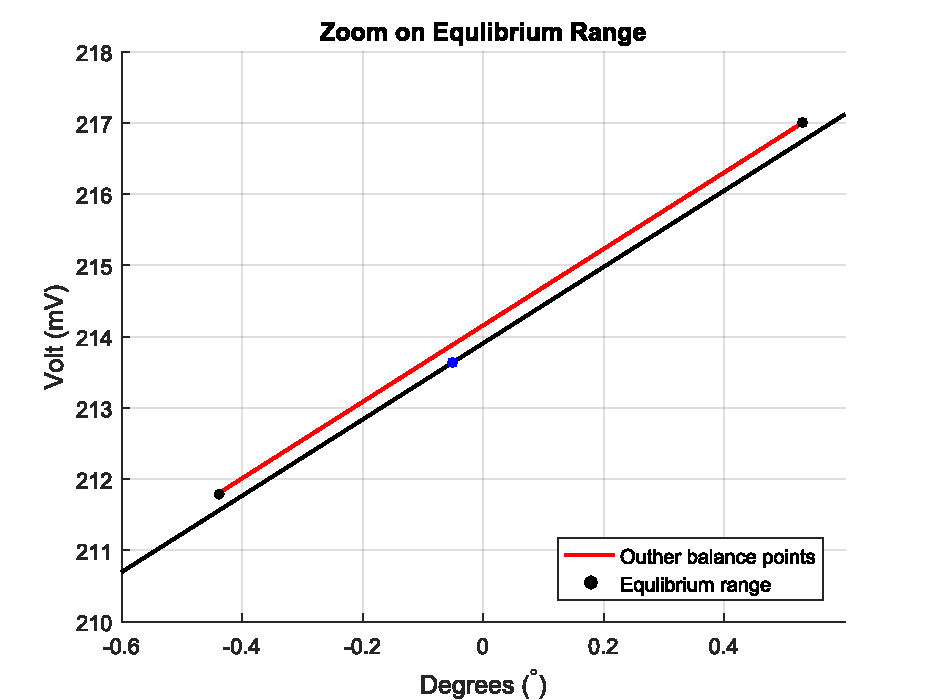
\includegraphics[scale=0.7]{figures/linearityOfPotmeterTest2-2}
	\caption{Raw test data plot}
	\label{linearityOfPotmeterTest2-2}
\end{figure}
Since the frame is connected to the baseframe through the potentiometer and the potentiometer is kept in place by bearings, the only force keeping the frame standing is the friction in the bearings and potentiometers.


